\chapter{Accessibility}
\label{ch:accessibility}
% ##################################################################################################################

\hfill \textbf{Author:} Dominik Ziemke

\begin{center} 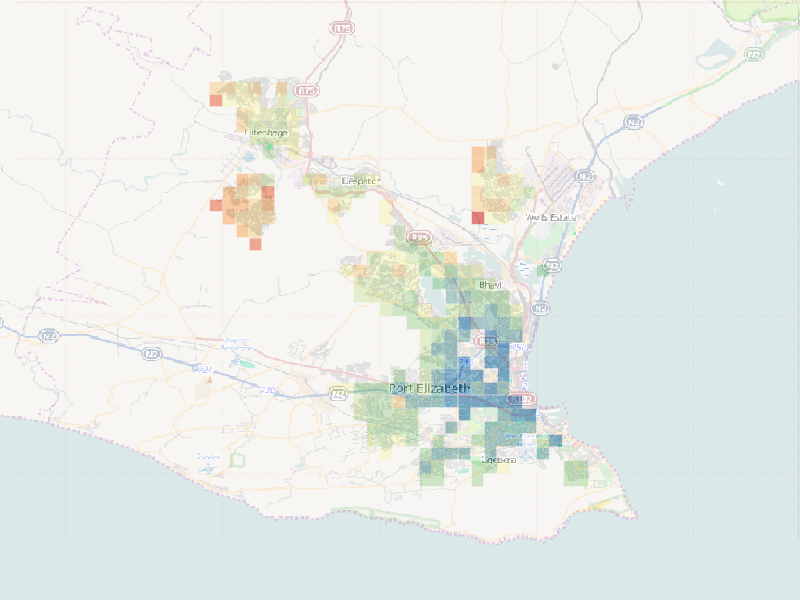
\includegraphics[width=1.\textwidth, angle=0]{extending/figures/accessibility/w_freeSpeed_snapshot.png} \end{center}

\createStandardInformation{accessibility}{\lstinline{RunAccessibilityExample} class}{accessibility}{\citet{NicolaiNagel2012HiResAccessibilityMethodInBook}}

% ##################################################################################################################

\mnote{wider context}
In transport science and planning, the term accessibility can refer to at least three different things. 
First, accessibility may be used to describe how well a certain component of the transport infrastructure 
is useable by citizens, in particular by handicapped people (Faura2012AccessibilityEvaluationTrafficSImulation). 
In this sense, \textit{accessibility guidelines} tell engineers and planners how to design transport 
infrastructure elements, such as public transport facilities, to make them accessibile to, i.e. useable 
by, all citizens. Second, accessibility may be used to describe how easy and convenient the approach 
towards a given land-use facility is. There are, for instace, studies (Fujiyama2004AccessibleDesignPTFacilities) 
that seek to improve the accessibility of shopping centers by redesigning the access roads and their 
connection to major roads. Finally, the term accessibility can be used from a more global perspective to 
describe the availability and spatial distribution of activity facilities within a given area, e.g. a 
metropolitan region, and the ease with which these facilities can be reached from other locations of 
the region. The accessibility extension of \gls{matsim} is concerned with this notion of accessibility. 
Its discussion in this chapter draws on \citet{NicolaiNagel2012HiResAccessibilityMethodInBook}.


\section{Introduction}
The improvement of accessibility is often stated as a central goal of proposed transport or infrastructure 
schemes \citep{GeursEtAl2012AccessibilityTransportIntroduction}. Not in all contexts, in which the term 
accessibility is discussed, however, it used as a precisely-definded, quantitative measure. While Batty 
\citep{Batty2009} traces the origins of the concept of accessibility back to location theory and regional 
economic planning of the 1920s when transport planning began in North America \citep{GeursEtAl2012AccessibilityTransportIntroduction}, 
Hansen, with his widely-cited 1959 paper \citep(Hansen1959), is generally credited for the first real 
definition of accessibility. He defines accessibility as \textit{the potential of opportunities for interaction} 
%also said so e.g. in Gulhan p.130
A bit more illustrative, \citet{DalviMartin1976...} define acessibility as 'the ease with which any 
land-use activity can be reached from a location using a particular transport system’. \citet(Hansen1959) 
also appears to be the first to have developed a procedure for the quatitaive quantitative consideraton of 
accessibility.
%It is notable that the development of gravity models, which have since then been the most prominent and 
%widely-applied type of destination choice models, has originally been intertwined with quantitative 
%approaches to accessibility analysis (cite Hansen ?????).

\mnote{typology}
%Depending on the concrete definition of quantitative accessibility measures, the explanatory power of the 
%result varies widely. As pointed out by \citet{GeursRitsema2001AccessibilityMeasures} (\citep[see also][]{Geurs2004AccessibilityReview}), quantitative indicators can rely on the following approaches:
In their widely-cited review, \citet{Geurs2004AccessibilityReview} identify four components of accessibility 
from different existing definitons and applied measures of accessibility that they consider important from a 
theoretical point of view:

\begin{enumerate}
	\item The \textbf{land-use} component reflects
	the number and spatial distribution of opportunities.
	
	\item The \textbf{transport} component describes the effort
	to travel from a given origin to a given destination.
	
	\item The \textbf{temporal} component considers the availability of activities at
	different times-of-day, \eg in the morning peak hours.
	
	\item The \textbf{individual} component addresses the different needs and
	opportunities of different socio-economic groups, \eg different income groups.
\end{enumerate}

%\begin{enumerate}
%\item An \textbf{activity-based} or \textbf{land-use-based} approach focuses on
%the distribution of possible activity locations (land use). One can, for instance,
%base calculations on the number and spatial distribution of activity opportunities
%like shopping locations or workplaces within a certain distance.
%%
%\item An \textbf{in\-fra\-struc\-ture-based} or \textbf{transport-based} approach takes into account the effort 
%to travel from a given origin to a given destination and 
%can be based on performance characteristics of the transport system, e.g. the
%average speed by mode at certain locations. If one considers, for instance, the
%number of shopping locations or workplaces under a defined travel time threshold,
%the activity-based and the infrastructure-based approaches can be combined.
%%
%\item A \textbf{temporal} component, which considers the availability of activities at
%different times-of-day, may be added.
%%
%\item An \textbf{individual} approach to accessibility computations can be
%obtained by addressing different needs and opportunities of different socio-economic groups, \eg different income groups.
%%
%\item A \textbf{utility-based} measurement of accessibility reflects the
%(economic) benefits, as the maximum expected utility, that someone gains
%from access to spatially distributed opportunities
%\citep{GeursRitsema2001AccessibilityMeasures,deJongEtAl2007LogsumTRA}. The
%typical example is the logsum term, which is discussed further below.
%\end{enumerate}

In this review, \citet{Geurs2004AccessibilityReview} mention and summarize various approaches applying the concept 
of accessibility, which have their focus on different of the aforementioned components of accessiblity:

\begin{enumerate}
	\item \textbf{Infrastructure-based} measures focus on the (observed or simulated) performance or service level 
	of transport infrastructure, \eg represented as average travel speed. These kind of measures are typically used 
	in transport planning.
	
	\item \textbf{Location-based} measures describe the level of accessibility to spatially distributed activities, such as 
	the number of jobs within 30 min travel time from origin locations. These kind of measures are typically used 
	in urban planning and geographical studies.
	
	\item \textbf{Person-based} measures analyze accessibility at the individual level, such as the activities in which an 
	individual can participate at a given time. These kind of measure are founded in the space–time geography 
	of \citet{Haegerstrand1970}.
	
	\item \textbf{Utility-based} measures analyze the economic benefits that people derive from access to spatially 
	distributed activities. These kind of measure have their origin in economic studies.
\end{enumerate}

\citet{Geurs2004AccessibilityReview} intersect these typical approaches with the four coponents of accessibility identified 
above, which leads to a matrix. This matrix illustrates how each of the four aforementioned compoments of accessibility is 
typically represented in the four different accessibility measures, where each measure is typically concerned with certain weaknesses 
concerning those accessibility components, which are not the particular focus of the given kind of measure. Accordingly, \citet{Geurs2004AccessibilityReview} assert that it would be desireable if an accessibility measure included 
all four aforementioned components of accessibility. The accessibility extension of \gls{matsim}, as will be described in 
the following, can be seen as an approach to achieve this goal.

\mnote{latest research}
In other recent strands of research, as identified by \citet{GeursEtAl2012AccessibilityTransportIntroduction}, encompass (among 
others) the concept of accessibility is also used for to the analysis of social exclusion (\eg by examining the benefit 
disadvantaged populations by comparing employment accessibility before and after the implementation of a transport scheme), 
the economic valuation of accessibility effects (\eg in cost-benefit analyses and studies assessing the impact of changes in 
public transport accessibility on house prices), and the analysis of behavior with accessibility mesures (\eg walking behavior 
dependent on different qualities of residential neighbourhood accessibility). 


\section{(Basic) Application OR Potential accessibility} LAND-USE COMPONENT
\mnote{measures in practice}
Today, methods to assess the quality of accessibility
%(cite BBSR, TUHH, TUM, Curtis, ... ??????????)
are often used in superordinate planning procedures like regional transport planning, where a central goal is to provide 
citizens with a certain quality of access to various services. For instance, the approach used by Germany's agency 
responsible for regional planning calculates travel times to major service facilities like airports or hospitals \citep{BBSR20xxErreichbarkeitsmodell}. %(\url{http://www.bbsr.bund.de/BBSR/DE/Raumbeobachtung/UeberRaumbeobachtung/Komponenten/Erreichbarkeitsmodell/erreichbarkeitsmodell_node.html}),
The results, typically visualized by mulit-colored maps, give useful insights into the supply of the population with 
certain services and can therefore assist the planning of the (transport) infrastructure in light of the goal to improve 
this supply. Since in this approach travel times to the \textit{next} airport, to the next hospital, and to the next 
autobahn access are caluclated, the implicit assumption is made that citizens' needs are fulfilled by one (i.e the \textit{next} 
or closest in terms of travel times) facility of a given type.

transport component

An accessibility measure becomes insightful, however, if not only the impedance to reach \textit{the nearest} facility 
serving a particular need is taken into account, but instead a set of multiple reachable facilities serving the same 
need is considered. This is due to the fact, that different facilities of the same type may offer a given service in 
different qualities. Also, services may become more beneficent when combined with complementary services provided by 
another facilities of the same type. For instance, a person wishing to make a holiday trip by airplane will likely 
take into account several airports in her/his vicinity when planning a journey instead of just looking at the flights 
offered from the nearest airport. Therefore, the accessibility to airports should be made dependent on the impedances 
to reach all of these airports instead of just the impedance to reach the nearest one. Facilities offering medical 
services may serve as another example. Only taking into account the nearest hospital may be sufficient when looking 
at siple services like first aid, which can be assumed to be available at almost \textit{any} hospital. In other cases, 
however, the supply with medical services will be better represented by considering several hospitals in the vicinity 
because they are likely to offer different kinds of medical treatment that complement each other. By considering various 
facilities of a given kind, the 

land-use component

An approach that pursues the idea of taking into account the whole scope of potential activity facilities is the one 
developed in Hansen's early study \citep{Hansen1959}, where an accessibility 
measure referred to as \textit{potential accessibility} is defined. It is specified as the (weighted) sum over the 
accessibilities of several facilities of a given type and is of the mathematical form
%The (quantitative) accessibility measure in the MATSim accessibility extension is of the mathematical form
\begin{equation}
	A_i = g\Big( \sum_j a_j \, f(c_{ij}) \Big) \ ,
	\label{eq:accessibility:basic}
\end{equation}
where the sum goes over all possible destinations (opportunities) $j$, $a_j$ is an indicator of the attractiveness of 
the opportunity, $c_{ij}$ is the generalized cost of travel to get from $i$ to $j$, $f(c)$ is an impedance function that 
typically decreases with increasing distance, and $g(.)$ is an arbitrary, but typically monotonically increasing, function. 
That is, the accessibility at $i$ is computed from a weighted sum over all possible destinations, where the weight is the 
product of the destination's attractiveness and the ease to get there. The (quantitative) accessibility measure used 
in the \gls{matsim} accessibility extension is of this mathematical form and may thus be seen 
as a \textit{potential accessibility} measure.

\mnote{ingoing vs. outgoing accessibility}
At this point, it may be important to note that the above-defined measure quantifies how good the accessibility \textit{to} 
certain services from a given location $i$ as the origin is. This kind of accessibility may therefore be referred to 
as ``outgoing'' accessibility, while a measure of ``ingoing'' accessibility would quantify how well a given destination 
location $j$ is accessible \textit{from} other locations. \citet{NicolaiNagel2012HiResAccessibilityMethodInBook} 
discuss under which circumstances both measures are interchangeable.

%TRASNPORT COMPONENT ----------------------------

\subsection{Accessibility Computation integrated with Transport Simulation}


\mnote{uncongested vs. congested network}
As mentioned above, accessibility computations are oftentimes based on travel times, which serve as an impedance 
measure. The calculation of these travel times can, however, vary. The most simple approach to calculate a travel time 
between two locations is measuring the Euclidian distance (beeline distance) between these two locations and then, 
by means of some kind of average speed, approximate the travel time between these two locations. Accoring to 
\citet{Geurs2004AccessibilityReview}, this is the usual approach in location-, person-, and utility-based accessibility 
approaches, i.e. those approaches where the focus is not explicitly on the considereation of the transport system.

To make the accessibility measure sensitive to transport infrastructure changes, a better representation of the travel 
impedance betwen origins and destinations is required. The most common approach appears to be the calculation of travel 
times by shortest-path algorithms on a network representation of the real-world transport infrastructure, as \eg done by \citet{BBSR20xxErreichbarkeitsmodell}.
%(\url{http://www.bbsr.bund.de/BBSR/DE/Raumbeobachtung/UeberRaumbeobachtung/Komponenten/Erreichbarkeitsmodell/erreichbarkeitsmodell_node.html})
Many accessibility computations are embedded into GIS software which offer respective procedures for network-based 
computations. The accessibility computation in \gls{matsim} offers this type of computation as well. To run it, an 
accessibility controller listener needs to be added to the \gls{matsim} controller. As input files, a network and a 
facilities file are necessary. An example for this application is given in (link to the RunAccessibilityComputation 
class already mentioned).

This may be regarded as a supply-based appraoch, since transport supply and the supply with activity opportunities are 
taken into account. The utilization of these two supply dimension by users are, however, not considered so far.

Therefore, no effects 
of competition, neither for the resources of the transport infrastructure (defined by network capacities) nor capacities 
of activity facilities, are taken into account. It is obvious, however, that these effects are relevant, as opportunities 
may become unavailbale to citizens if they cannot be reached anymore due to overly high travel times on the network or 
in cases where capacities of activity facilities are exceeded. The latter can in principle be adressed by specifying 
facility capacities in the accorinding value in the facilities input file. The according code adaption for observing 
these capacities is currently underway  (???). Network capacities and their effects on the adaption of agents' behavior 
are considered by the \gls{matsim} transport simulation (see chapter ?????? of this book)

%explained in the next section....
%\subsection{Accessibility Computation integrated with Transport Simulation}
%In order to observe capacity restriction of the transport network and of activity facilities and the impacts of this 
%effects on the demand and respective changes in levels of accessibilities, 

In order to take these effects into account, the \lgs{matsim} accessibility extension 
needs to be run with a \gls{matsim} transport simualtion

%(in the example described above in section "basic application", \gls{matsim} has only been used to provide the 
%infrastructure for the accessibility computation, while no actual simulation has been performed).

As stated in section ?????????, the expressiveness of the accessibility calculation can be significantly increased 
by taking into account (transport and activity) demand next to the considertation of the supply side (transport 
infrastructure and supply with spatially distrubuted activity facilieites). 

This is also one major argument for the 
integration of an accessibility computation with the dynamic transport simulation system \gls{matsim}. While other 
accessibility tool, of which the majority is based on GIS systems, offer opportunites to calculate travel times on 
a routed network, they are not able to calculate accessibility changes dependent on the interaction of supply and 
demand. 

Network travel times may be dependent on time of day in that \eg peak- or off-peak travel times may be 
considered. A more detailed consideration of temporal effects is, however, only possible when the accessibility 
computation is coupled with a dynamic traffic simulation. (?????????????)


=======
\subsection{Accessibility and Transport Simulation}
In order to observe capacity restriction of the transport network and of activity facilities and the impacts of 
this effects on the demand and respective changes in levels of accessibilities, the \gls{matsim} accessibility 
extension needs to be run with a \gls{matsim} transport simualtion (in the example described above in section "basic 
application", the \gls{matsim} has only been used to provide the infrastructure for the accessibility computation, 
while no actual simulation has been performed).

performance of the transport system is obviously dependent of the utilization of transport supply by transport 
demand. With increasing travel times, for instance, the accessibility of a given location may decrease. To be able 
to analyze such effects, a transport simulation which represents the interaction of transport supply and demand is 
needed. This is one major argument why it is reasonable to integrate an accessibility extension into the MATSim framework.
=======
As stated in section ?????????, the expressiveness of the accessibility calculation can be significantly increased 
by taking into account (transport and activity) demand next to the consideration of the supply side (transport 
infrastructure and supply with spatially distrubuted activity facilieites). This is also one major argument for 
the integration of an accessibility computation with the dynamic transport simulation system \gls{matsim}. While 
other accessibility tool, of which the majority is based on GIS systems, offer opportunities to calculate travel 
times on a routed network, they are not able to calculate accessibility changes dependent on the interaction of 
supply and demand. (?????????????)

This is possible in \gls{matsim} can also be done in MATSim by adding an accessibility controller listener to the 
controller and only network and facilities files

Equally, the interaction of supply and demand concerning the uasge of activity facilities can be considered in 
the \gls{matsim} accessibility extension. To do so, facilities in the facilities input file need to be equipped 
with according facilities capacities.

This way, the accessibility computation can be made dependent upon time-of-day, which is useful in contexts were 
levels of transport demand varies significantly over the course of the day as, for instance, in contexts where 
pronounced morning and afternoon peaks exist. This way, accessibility changes related to transport policies and 
corresponding reaction of decision makers can be considered in a more comprehensive fashion.

\mnote{spatial resolution, zones vs. points}

LAND-USE COMPONENT

In contrast to many other transport simulations, \gls{matsim} is not zone-based, but based on coordinates (see 
chapter ????? of this book). Therefore, the accessibility computation within MATSim can also be conducted independent 
of any zonation system and, instead, be based on points or on a raster with arbitrary granularity. This avoids 
several issues that may arise if accessibility computations are based on zones 
(see \citep[e.g.,][]{NicolaiNagel2012HiResAccessibilityMethodInBook}) as it is done by other quantitative 
accessibility computations 
%
%\citep[e.g.][]{Curtis, BBSR , LiuZhu2004AccessibilityAnalyst} (?????)
\ah{temporarily commented out as it kills the continous integration: \url{http://ci.matsim.org:8080/view/All/job/MATSim-Book/ws/}}
%
(\url{http://www.bbsr.bund.de/BBSR/DE/Raumbeobachtung/UeberRaumbeobachtung/Komponenten/Erreichbarkeitsmodell/erreichbarkeitsmodell_node.html}). Being raster- or coordinate-based, the outcome of the MATSim accessibility computation can be considered as 
an accessibility field,
\ie as a measure continuously varying in space, $A(x,y)$, where $x$ and $y$
are the coordinates. As is common in many areas of science, such
fields can be visualized by calculating the values on regular grid
points and using an averaging plotting routine (?????????). An example of such a visualization is shown in figure ????.

To use this functionality a GridBasedAccessibilityControllerListener needs to be added to the controller.

Alternatively, if the calculation based on some given zonation system is desidered, the ZoneBasedAccessibilityControllerListener can be used.




#############################

???????????????
This appears plausible when cosidering, for instance, the well-known transport-land-use cycle that describes the 
bidirectional interrelationship between transport and land use. Considering these mechnism, ?????? 

Curtis et al. (cite Curtis... ??????) also argue that accessibility-based analysis methods may be suitable to overcome 
the deficits that traditional transport analysis methods possess in terms of analyzing transport policies that are not 
construction-based like transport demand management schemes.
###############################





\section{Econometric Interpretation????}

\mnote{econometric interpretation} 
As pointed out by Curtis (????????????????) accessibilities can serve as an evaluation measure for transport 
policies. While most measures today rely on pure infrastructure characteristics (cite ??????????? look in ERAfrika-Antrag), 
accessibility indicators are a holistic measure, which explicitly observes the interrelationship between transport and land use.
TRANSPORT AND LAND USE ----------------------------------------

To make the quantitative accessibility measure most expressive in terms of econometric evaluation (e.g. cost-benefit 
analyses), it seems sensible to adapt equation \ref{eq:accessibility:basic} as 
follows: $g(.) = \ln(.)$, $a_j = 1$, $f(c_{ij}) = e^{-c_{ij}}$, and $-c_{ij} = V_{ij}$. Thus, 
equation \ref{eq:accessibility:basic} becomes
\begin{equation}
	A_i := \ln \sum_k e^{V_{ik}} \ ,
	\label{eq:accessibility:logsum0}
\end{equation}
where $k$ goes over all possible destinations, and $V_{ik}$ is the
disutility of travel in order to get from location $i$ to location
$k$. Equation \ref{eq:accessibility:logsum0} is the so-called logsum term and has an econometric interpretation 
as the expected maximum utility \citep[e.g.][]{Ben-AkivaBook}. It can be derived as follows: Assume that the full 
utility of location $k$, seen from $i$, is $U_{ik} = V_{base} + V_{ik} + \epsilon_{ik}$, where $V_{base}$ is a constant 
base utility for doing the activity at any location, $V_{ik}$ is the systematic ($=$ observed) disutility to travel to 
location $k$, and $\epsilon_{ik}$ is a random term which picks up the randomness of the travel disutility and, more 
importantly, also the utility fluctuations around $V_{base}$.  Under the typical assumption that the $\epsilon_{ik}$ 
are independent and identically Gumbel-distributed random variables, the expectation value of $U_{ik}$ becomes
\begin{equation}
	E(U_i) = E(\max_k U_{ik}) = \ln \sum_k e^{V_{ik}} + Const \equiv A_i + Const \ .
\end{equation}
$Const$ is an integration constant, which can be dropped as it is the same for all locations. $A_i$ may also be negative.

\citet{GeuersEtAl20xx}, for instance, use the logsum measure of user benefits as an alternative to the travel time 
savings method (i.e. rule-of-half measure) in a case study, where they examine the effects of spatial planning on 
the accessibility benefits and the economic efficiency of public transport projects.

%In Chapter 8, Karst T. Geurs, Michiel de Bok and Barry Zondag examine the degree to which spatial planning affects 
%the accessibility benefits and economic efficiency of public transport projects. As a case study, plans for a large 
%urban planning project in the Netherlands are examined, combined with major rail investment alternatives (involving 
%the upgrade of an existing bridges and construction of new bridges). The authors apply the logsum measure of user 
%benefits, as an alternative to the travel time savings method (i.e. rule-of-half measure)

%the major disadvantages of utility-based measures are the difficult interpretability and communicability (Geurs p136)


\section{Computational Aspects}

\mnote{functionings}
The concrete calculation of the accessibility $A_i$ of a given origin location $i$ to opportunity locations $k$ works as 
follows: The origin location $i$ and opportunity locations $k$ are assigned to a congested road network with time dependent 
travel times as it is simulated in MATSim. For every $i$ a so-called ``least cost path tree'' computation runs through the 
network and determines the best route, and thus the least negative travel utility $V_{ik}$, to each opportunity location 
$k$ by using Dijkstra's shortest path algorithm \citep{Dijkstra1959ShortestPath}. The best route from $i$ to $k$ depends 
on the given generalized cost such as link travel times or distances. Once the least cost path tree has explored all 
nodes, the resulting disutilities $V_{ik}$ for all opportunities are queried and the accessibility is calculated as 
stated in Equation~(\ref{eq:accessibility:logsum0}).


USAGE: controlerListener in MATSim; if various activities and various modes are considered, one such contoler listener 
is added for each combination


\mnote{computational aspects}
TODO: say something about computation characteristics

runtime optimization

\mnote{resolution}
resolution can in principal be increased infinitely. Because of the runtime optimization, computation time increases 
sub-linearly with resolution.

studies showed that no significant further insights can be gained by increasing the resolution beyond 100\,meters.

\mnote{other}
ADD: different modes, activities

ADD: transport/land-use interaction

automatic

microscopic




In Chapter 7, Tijs Neutens applies a combination of place-based and person-based measures of accessibility to achieve 
a rich portrayal of accessi- bility to public service delivery. A case study of accessibility to government offices 
in the city of Ghent (Belgium) illustrates complementary insights related to service delivery. Three specific aspects 
of accessibility are studied: spatial proximity, spatial choice and scheduling flexibility.

Chapter 14, Derek Halden explains some of the experiences, pitfalls and lessons learned in 20\,years of accessibility 
planning in the UK The accessibility planning approach is able to frame the transport plan- ning dialogue within 
the transport user language 


\section{Data}
\mnote{data}
free data

the accessibility computation does not rely on specific local data, that need to be collected, prepared and processed. 
Instead, it relies on data form \gls{osm} (include link...?) which is openly and freely for every region in the world, 
and also has the same data format world-wide

\mnote{applicability, useability}

TRANSPORT-LAND-USE-CYCLE

\mnote{advantages over GIS-baed tools}
HOW WELL CAN THE TRANSPORT SYSTEM BE REPRESENTED IN GIS?




\section{Conclusion}
There are many different approaches to calculate accessibilities. As pointed out, most approaches focus on a particular 
componetn of accessibility, while other components that influence accessibility, if it is understood by Hansen's definition 
as the potential for interaction, are represented only in a limited way. For example, accessibility computations used in 
transport planning represent transport networks, and thus the transport componentn of accessibility very well, do, however, 
mostly not represent properties of facilities or temporal effects. As pointed out by Geurs???????, it is desirbale if an 
accessibility computation consideres all components of accessibility (the tranpsort, the land use, the temporal and the 
individual component) well. The accessibility extension of \gls{matsim} can be seen as an approach to achieve this. First, 
the dynamics of the transport system are represented via the dynmic traffic simulation. As \gls{matsim} is a simulation 
that runs second by second, the temporal dimension is reprenseted in a very detailed way. Accessibility computations in 
\gls{matsim} can be dependent on a arbitrary simulation time. Via the integration of the accessibility computation with 
the microscopic simulation of individual agents who follow individual day plans (sequences of activities whioch they 
wish to pursue), the individual component is also represented in \gls{matsim} to a high degree.

location-based... activity facilities

Actual accessibility values calculated by the \gls{matsim} accessibility extension are of the form of \textit{potential 
	accessibility measure} as originlally defined by Hansen. This way, results can be interpreted as logsum values, 
which makes them suitable to be used for economic evaluations like benefit-cost analyses as it has already been done 
by other authors.

%Aufgabe des Staates: Grundversorgung der Bevölkerung
%Nötig: (Infrastruktur-)Maßnahmen bewerten
%Heute i.d.R. ausschließlich auf Basis verkehrs- und mobilitätsbezogener Maße
%Qualität der erreichbaren Angebote
%Nicht bewertet
%Mittels Durchschnittswerten bewertet
%Keine Aussage bzgl. etwaiger räumlicher und/oder sozialer Ungleichverteilungen
%Verteilungsmaße (z.B. generalisierter Gini-Koeffizient)
%Verortung unterversorgter Personen?
%Beitrag zur Verbesserung des Zugangs zum jeweiligen Angebot?



public GridBasedAccessibilityControlerListenerV3(ActivityFacilities opportunities, Config config, Network network)

\section{Invocation}

\subsection{Minimal}

...



\subsection{Invocation as ``Script in Java''}

See \url{http://matsim.org/javadoc} $\to$ accessibility $\to$ \lstinline{RunAccessibility} class for an example.



% ##################################################################################################################

% Local Variables:
% mode: latex
% mode: reftex
% mode: visual-line
% TeX-master: "../../main"
% comment-padding: 1
% fill-column: 9999
% End: 
